\chapter{Introduction}
\label{chp-introduction}

% Sample content:
% \lipsum[1-2]

\begin{figure}
  \centering
  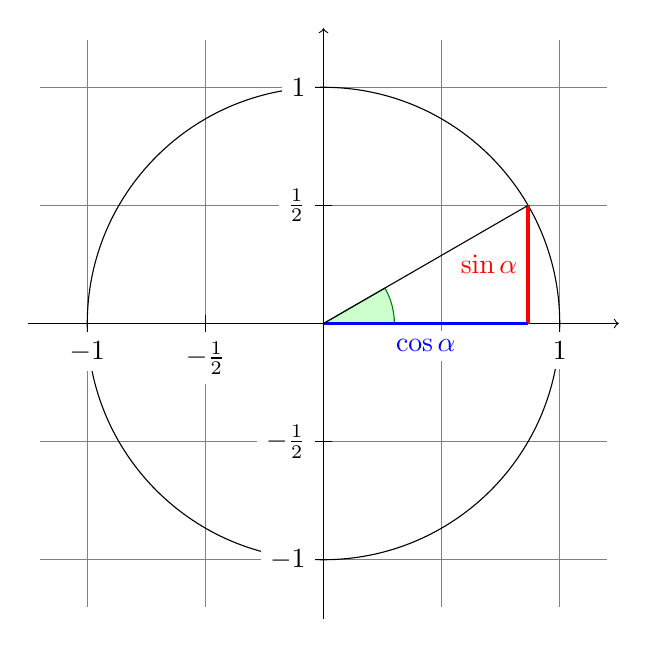
\begin{tikzpicture}[scale=3]
    \draw[step=.5cm, gray, very thin] (-1.2,-1.2) grid (1.2,1.2); 
    \filldraw[fill=green!20,draw=green!50!black] (0,0) -- (3mm,0mm) arc (0:30:3mm) -- cycle; 
    \draw[->] (-1.25,0) -- (1.25,0) coordinate (x axis);
    \draw[->] (0,-1.25) -- (0,1.25) coordinate (y axis);
    \draw (0,0) circle (1cm);
    \draw[very thick,red] (30:1cm) -- node[left,fill=white] {$\sin \alpha$} (30:1cm |- x axis);
    \draw[very thick,blue] (30:1cm |- x axis) -- node[below=2pt,fill=white] {$\cos \alpha$} (0,0);
    \draw (0,0) -- (30:1cm);
    \foreach \x/\xtext in {-1, -0.5/-\frac{1}{2}, 1} 
    \draw (\x cm,1pt) -- (\x cm,-1pt) node[anchor=north,fill=white] {$\xtext$};
    \foreach \y/\ytext in {-1, -0.5/-\frac{1}{2}, 0.5/\frac{1}{2}, 1} 
    \draw (1pt,\y cm) -- (-1pt,\y cm) node[anchor=east,fill=white] {$\ytext$};
  \end{tikzpicture}
  \caption{A pictorial view of \refThm{thm-pythagorean}.}
  \label{fig-pythagorean}
\end{figure}

\begin{definition}
  A function $f$ is said to be \emph{continuous} if its derivative exists at every point.
\end{definition}

\begin{lemma}
  Let $f$ be a function whose derivative exists in every point, then $f$ is 
  a continuous function.
\end{lemma}

\begin{theorem}[Pythagorean theorem]
  \label{thm-pythagorean}
  This is a theorema about right triangles and can be summarised in the next 
  equation 
  \[ x^2 + y^2 = z^2 \]
\end{theorem}
\begin{proof}
  I have discovered a truly marvelous proof of this, which this margin is too narrow to contain.
\end{proof}

And a consequence of \refThm{thm-pythagorean} is the statement in the next 
corollary~\cite{he2017physhare}.

\begin{corollary}
  There's no right rectangle whose sides measure 3cm, 4cm, and 6cm.
\end{corollary}

% \lipsum[3-5]

\begin{table}
  \centering
  \caption{Predicted final standings of Group B.}
  \begin{tabular}{l*{6}{c}r}
    Team              & P & W & D & L & F  & A & Pts \\
    \hline
    Manchester United & 6 & 4 & 0 & 2 & 10 & 5 & 12  \\
    Celtic            & 6 & 3 & 0 & 3 &  8 & 9 &  9  \\
    Benfica           & 6 & 2 & 1 & 3 &  7 & 8 &  7  \\
    FC Copenhagen     & 6 & 2 & 1 & 3 &  5 & 8 &  7  \\
  \end{tabular}
  \label{tab-forecast}
\end{table}

\lipsum[5-7]